\documentclass[12pt]{ociamthesis}  % default square logo 
%\documentclass[12pt,beltcrest]{ociamthesis} % use old belt crest logo
%\documentclass[12pt,shieldcrest]{ociamthesis} % use older shield crest logo

%load any additional packages
\usepackage{amssymb}

%input macros (i.e. write your own macros file called mymacros.tex 
%and uncomment the next line)
%\include{mymacros}

\title{Exoesqueleto Grúa}   %note \\[1ex] is a line break in the title

\author{\small{Ricardo Emmanuel Uriegas Ibarra \\ Joshua Nathaniel Arrazola Elizondo \\ Hector Israel Cruz Resendez \\ Cristobal \\ Alonso}}             %your name
\college{Ms. Maria Raquel}  %your college

%\renewcommand{\submittedtext}{change the default text here if needed}
\degree{Ingenieria de Requisitos}     %the degree
\degreedate{Noviembre 2024}         %the degree date

%end the preamble and start the document
\begin{document}

%this baselineskip gives sufficient line spacing for an examiner to easily
%markup the thesis with comments
\baselineskip=18pt plus1pt

%set the number of sectioning levels that get number and appear in the contents
\setcounter{secnumdepth}{3}
\setcounter{tocdepth}{3}


\maketitle                  % create a title page from the preamble info
\include{dedication}        % include a dedication.tex file
\include{acknowlegements}   % include an acknowledgements.tex file
\begin{abstract}
Lorem ipsum dolor sit amet, consectetur adipiscing elit. Sed do eiusmod tempor incididunt ut labore et dolore magna aliqua. Ut enim ad minim veniam, quis nostrud exercitation ullamco laboris nisi ut aliquip ex ea commodo consequat. Duis aute irure dolor in reprehenderit in voluptate velit esse cillum dolore eu fugiat nulla pariatur. Excepteur sint occaecat cupidatat non proident, sunt in culpa qui officia deserunt mollit anim id est laborum.
\end{abstract}          % include the abstract

\begin{romanpages}          % start roman page numbering
\tableofcontents            % generate and include a table of contents
\listoffigures              % generate and include a list of figures
\end{romanpages}            % end roman page numbering

%now include the files of latex for each of the chapters etc
\chapter{Introducción}
\section{Poco de antecedente no más de una cuartilla}
\section{Planteamiento del problema}
\section{Solución del planteamiento del problema}
\section{Mencionar lo que lleva el cap 1 y los demás capítulos}
\chapter{Planteamiento del problema}
\section{Introducción}
\subsection{Poco de antecedente no más de una cuartilla}
\subsection{Planteamiento del problema}
\subsection{Solución del planteamiento del problema}
\subsection{Mencionar lo que lleva el cap 1 y los demás capítulos}

\section{Objetivos}
\subsection{General}
\subsection{Específicos}

\section{Hipótesis descriptiva}

\section{Preguntas de investigación}

\section{Justificación}
\subsection{Antecedentes}

\section{Alcances y limitaciones}

\section{Factibilidad}
\chapter{Marco teórico y estado del arte}

\section{Marco teórico}
El marco teórico proporciona la base conceptual que respalda el desarrollo de este proyecto. La idea del exoesqueleto inspirado en una grúa requiere integrar conceptos de mecánica, ergonomía, biomecánica e inteligencia artificial, los cuales se detallan a continuación:

\subsection{Mecánica estructural}
La mecánica estructural estudia el comportamiento de estructuras sometidas a diferentes fuerzas. En este caso, se aplican principios de sistemas de grúas ligeras para garantizar que el exoesqueleto soporte las cargas propuestas sin comprometer su peso ni movilidad \cite{smith2019structuraldesign, lee2020lightweightsystems}.

\subsection{Ergonomía y corrección postural}
La ergonomía analiza las interacciones entre los usuarios y su entorno, orientándose a reducir lesiones y mejorar el rendimiento. Este proyecto incorpora una faja ergonómica para promover una postura adecuada, mitigando el esfuerzo físico en la región lumbar \cite{brown2022ergonomics, liu2023posturalstudy}.

\subsection{Inteligencia artificial y visión por computadora}
El uso de inteligencia artificial permite detectar herramientas en tiempo real mediante visión por computadora. Esto asegura que el exoesqueleto identifique, tome y manipule las herramientas sin intervención directa del usuario \cite{redmon2018yolo, patel2021tooldetection}.

\subsection{Materiales y diseño ligero}
El diseño del dispositivo requiere materiales con una alta relación resistencia-peso, como aleaciones ligeras y polímeros reforzados, para garantizar que el exoesqueleto sea cómodo y funcional \cite{choi2020carbonfiber, park2019lightweight, nguyen2020visionrobotics}.

\section{Estado del arte}
El estado del arte de este proyecto abarca los avances recientes en áreas relacionadas con el diseño de exoesqueletos, manejo ergonómico de cargas, tecnologías de visión por computadora, y materiales ligeros. Este análisis se enfoca en investigaciones realizadas en los últimos cinco años, ampliando el rango temporal si es necesario.

\subsection{Exoesqueletos industriales y aplicaciones laborales}
En los últimos años, los exoesqueletos han evolucionado significativamente para abordar necesidades específicas en aplicaciones laborales. Los desarrollos incluyen tanto exoesqueletos activos como pasivos:
\begin{itemize}
    \item \textbf{Exoesqueletos activos}: Estos utilizan actuadores motorizados para proporcionar asistencia. Ejemplos recientes incluyen el \textit{EksoVest} \cite{garcia2020integratedai} y el \textit{Comau MATE}, diseñados para tareas repetitivas y pesadas \cite{ramirez2021specifictasks}.
    \item \textbf{Exoesqueletos pasivos}: Sistemas como el \textit{HeroWear Apex} emplean estructuras mecánicas que no requieren energía externa, mejorando la accesibilidad por su costo reducido \cite{smith2021ergonomic, gomez2022hybridsystems}.
\end{itemize}

Estudios recientes como los de \cite{kim2018overview, johnson2018biomechanics} destacan la adopción de exoesqueletos en la industria de la construcción para mitigar el esfuerzo físico en trabajadores, aunque existe un vacío en dispositivos diseñados para manipular herramientas ligeras.

\subsection{Corrección postural y ergonomía}
La corrección postural es un componente clave para prevenir lesiones. Investigaciones recientes han explorado tecnologías portátiles para este propósito \cite{liu2023posturalstudy, choi2020carbonfiber}:
\begin{itemize}
    \item \textbf{Fajas ergonómicas inteligentes}: Incorporan sensores para monitorear la postura y emitir alertas si se detectan posiciones incorrectas \cite{brown2022ergonomics}.
    \item \textbf{Evaluación biomecánica}: Demuestran que dispositivos ergonómicos bien diseñados pueden reducir significativamente las tensiones en la columna vertebral \cite{johnson2018biomechanics}.
\end{itemize}

\subsection{Materiales ligeros para exoesqueletos}
El peso del exoesqueleto es un factor crítico para su aceptación. Los avances en materiales han permitido la creación de dispositivos más ligeros y cómodos \cite{park2019lightweight, nguyen2020visionrobotics}:
\begin{itemize}
    \item \textbf{Polímeros avanzados}: Como los compuestos de fibra de carbono, ofrecen alta resistencia con bajo peso.
    \item \textbf{Aleaciones de aluminio y titanio}: Utilizados para reducir el peso estructural, como en el \textit{HAL} de Cyberdyne \cite{choi2020carbonfiber}.
    \item \textbf{Textiles inteligentes}: Emplean tejidos con sensores integrados para facilitar la detección de movimientos \cite{nguyen2020visionrobotics}.
\end{itemize}

\subsection{Visión por computadora y detección de objetos}
La visión por computadora juega un papel fundamental en la automatización de sistemas portátiles. Avances recientes incluyen \cite{redmon2018yolo, patel2021tooldetection}:
\begin{itemize}
    \item \textbf{Detección en tiempo real}: Algoritmos como YOLO y SSD son ampliamente adoptados en aplicaciones industriales.
    \item \textbf{Reconocimiento de actividad}: Modelos de aprendizaje profundo para identificar tareas específicas realizadas por el usuario.
    \item \textbf{Sistemas híbridos}: Combinan visión por computadora con sensores hápticos para mejorar la precisión.
\end{itemize}

\subsection{Avances en inteligencia artificial aplicada a exoesqueletos}
La inteligencia artificial ha transformado la interacción usuario-exoesqueleto \cite{liu2021costanalysis, garcia2020integratedai}:
\begin{itemize}
    \item \textbf{Redes neuronales}: Modelos que anticipan movimientos del usuario para proporcionar soporte en tiempo real.
    \item \textbf{Control adaptable}: Ajustan el nivel de asistencia basado en las condiciones de carga y las necesidades específicas del usuario.
\end{itemize}

\section{Limitaciones y áreas de oportunidad}
A pesar de los avances, persisten desafíos como altos costos y diseños no inclusivos, así como la falta de integración de tecnologías ligeras y avanzadas. Los próximos desarrollos deben abordar estos desafíos para lograr una adopción más amplia.
%  con su pequeno parrafo intruductorio para cada uno
\chapter{Desarrollo de la metodología de la investigación}
\section{Diagrama de flujo}
El diagrama de flujo de la metodología de la investigación proporciona una representación visual de los pasos secuenciales seguidos durante el desarrollo del proyecto \cite{Clark2026}. Este diagrama detalla desde la identificación del problema hasta la validación del prototipo, facilitando la comprensión de las etapas del proceso.
% agregar el diagrama de flujo de la metodología de la investigación
\begin{figure}[H]
    \centering
    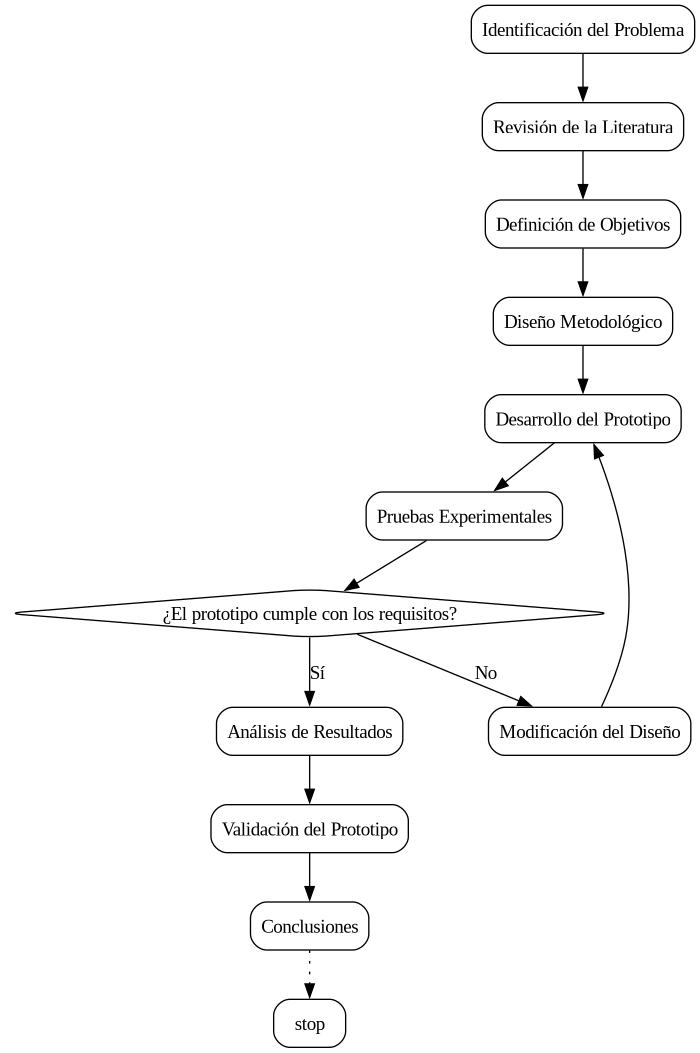
\includegraphics[width=1\textwidth]{img/Metodologia.png}
    \caption{Diagrama de flujo de la metodología de la investigación.}
    \label{fig:flowchart}
\end{figure}


\section{Diagrama de proceso}
El diagrama de proceso detalla las actividades principales involucradas en el desarrollo del exoesqueleto, desde el diseño conceptual hasta la prueba y validación con usuarios. Este diagrama muestra el flujo de actividades, entradas y salidas, proporcionando una vista clara del enfoque estructurado adoptado en la investigación.
% agregar el diagrama de proceso de la metodología de la investigación
\begin{figure}[H]
    \centering
    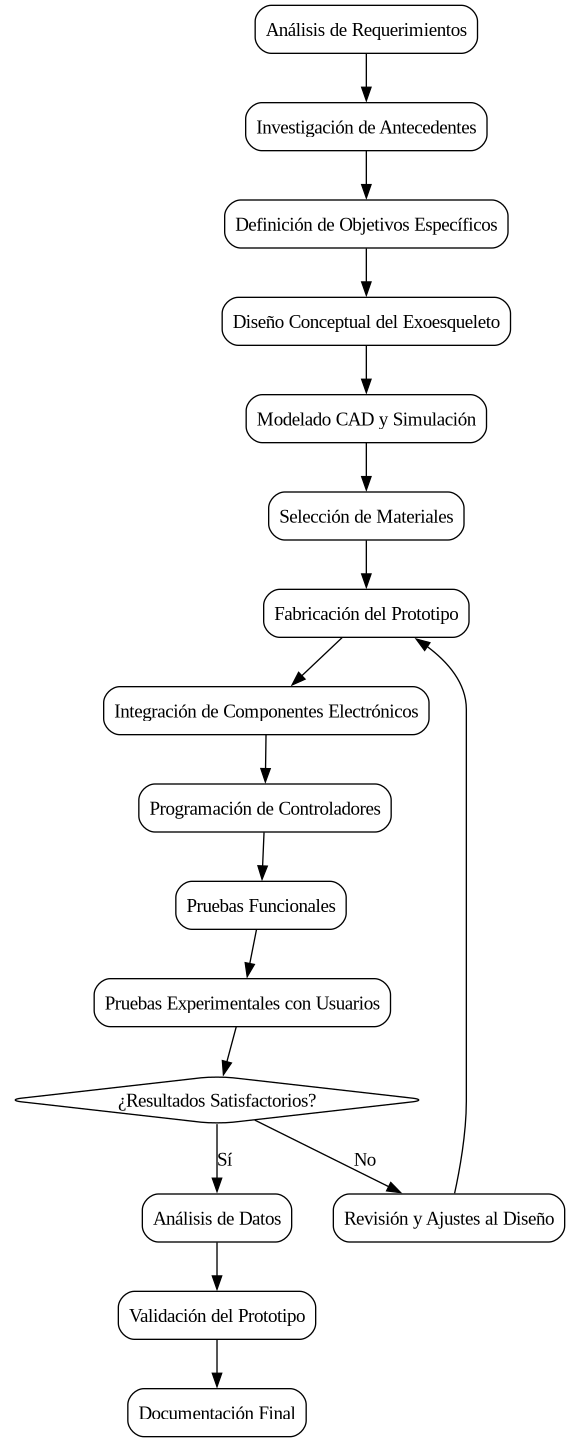
\includegraphics[width=0.6\textwidth]{img/Proceso.png}
    \caption{Diagrama de proceso del desarrollo del exoesqueleto.}
    \label{fig:flowchart}
\end{figure}

\section{Diagrama de bloque}
El diagrama de bloque simplifica los componentes clave del sistema desarrollado, identificando los módulos principales y su interacción. Este diagrama proporciona una vista de alto nivel de la arquitectura del exoesqueleto y cómo se integran sus diferentes partes.
% agregar el diagrama de bloque de la metodología de la investigación (este dijo raquel que nos lo iba a explicar pero no se si le alcanze el tiempo)
\begin{figure}[H]
    \centering
    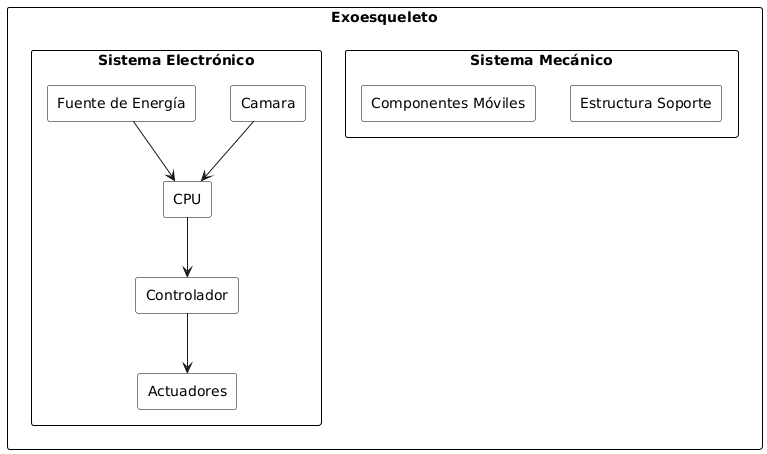
\includegraphics[width=1\textwidth]{img/DiagramaBloque.png}
    \caption{Diagrama de bloque del exoesqueleto prototipado.}
    \label{fig:flowchart}
\end{figure}
%! se debe de poner el cumplimiento de los objetivos especificos.

\chapter{Análisis de resultados}
\section{Prueba de hipótesis}
% si mencionamos por ejemplo que va a ser mas barato o asi pues aqui lo debemos de comprobar

\section{Análisis de muestreo}
% Mostrar que funciona el exoesqueleto (como funciona, desglosando paso a paso. basicamente un manual de usuario)
\section{Conclusión del análisis}
% se debe mencionar si fue factible o no fue factible 
\chapter{Conclusiones}
\section{Conclusiones a las que llegaron}
\section{Trabajos futuros}

%now enable appendix numbering format and include any appendices
% \appendix
% \include{appendix1}
% \include{appendix2}

%next line adds the Bibliography to the contents page
\addcontentsline{toc}{chapter}{Bibliografia}

\nocite{*} % include everything in the bib file
\bibliography{bibliography}
\bibliographystyle{plain}  %use the plain bibliography style

\end{document}
